\documentclass{beamer}
\DeclareFontShape{OT1}{cmss}{b}{n}{<->ssub * cmss/bx/n}{} 
\usetheme{default}
\usepackage{amsmath}
\usepackage{amsfonts}
\usepackage{mathbbol}
\usepackage{xcolor} % before tikz or tkz-euclide if necessary
\usepackage{tkz-euclide} % no need to load TikZ
\usepackage{multirow}
\usepackage{lmodern}
\usepackage{bm}
\usepackage{subcaption}

\usepackage[
backend=biber,
style=authoryear-icomp,
sortlocale=de_DE,
natbib=true,
url=false, 
doi=true,
eprint=false
]{biblatex}
\addbibresource{../../Bibliography/main_ML.bib}



\titlegraphic{
\includegraphics[width=2cm]{../../Figures/UAMS_RGB.png}
}


\title{Statistical Machine Learning\\ Finding Minima Algorithms}
\author{Horacio G\'omez-Acevedo\\ Department of Biomedical Informatics\\
	University of Arkansas for Medical Sciences}
\begin{document}
	\begin{frame}[plain]
		\maketitle
	\end{frame}
	
	\begin{frame}{Case $n=1$}
		Let's suppose we have a real valued function which is smooth $f\colon \mathbb{R}\to \mathbb{R}$. Then, we can approximate the function in a vicinity of $x=c$ by the so-called Taylor expansion
		\begin{equation*}
			f(x)= f(c)+ \frac{df}{dx}(c) (x-c)+  \frac{1}{2!} \frac{d^2f}{dx^2}(c) (x-c)^2 +  \frac{1}{3!} \frac{d^3f}{dx^3}(c) (x-c)^3+ \cdots
		\end{equation*}
		Notice that when $x$ is very close to $c$, then $(x-c)^p$ for $p\ge 3$ starts getting exceedingly small. Then, we write 
			\begin{equation*}
			f(x) \approx f(c)+ \frac{df}{dx}(c) (x-c)+  \frac{1}{2!} \frac{d^2f}{dx^2}(c) (x-c)^2 
		\end{equation*}
		
		If at the point $x=c$ the function reaches a (local) minimum, then $f'(c)=0$.
		
		
	\end{frame}

	\begin{frame}{Case $n\ge 2$}
	Let's suppose we have a real valued function which is smooth $f\colon \mathbb{R}^n\to \mathbb{R}$. Then, we can approximate the function in a vicinity of $x=c$ by the so-called Taylor expansion
	\begin{equation*}
		\begin{split}
	f(\textbf{x}) = &f(\textbf{c})+ \sum_i \frac{\partial f}{\partial x_i}(c) (x_i-c_i)+  \frac{1}{2!} \sum_{i,j}\frac{\partial^2f}{\partial x_i \partial x_j}(c) (x_i-c_i)(x_j-c_j) +\\
	&  +  \text{ higher order terms}\\
	\approx &f(\textbf{c})+ (\textbf{x}-\textbf{c})^T \nabla f(\textbf{c})+ \frac{1}{2} (\textbf{x}-\textbf{c})^T H_f(\textbf{c}) (\textbf{x}-\textbf{c})
		\end{split}
	\end{equation*}

	Where $H_f(\textbf{c})$ is the \textbf{Hessian matrix} defined as 
	\begin{equation*}
		H_f(\textbf{c})= \begin{pmatrix}
			\frac{\partial^2 f}{\partial x_1 \partial x_1} (\textbf{c}) & 	\frac{\partial^2 f}{\partial x_1 \partial x_2} (\textbf{c}) & \cdots & 	\frac{\partial^2 f}{\partial x_1 \partial x_n} (\textbf{c}) \\
				\frac{\partial^2 f}{\partial x_2 \partial x_1} (\textbf{c})  & 	\frac{\partial^2 f}{\partial x_2 \partial x_2} (\textbf{c}) & \cdots & 	\frac{\partial^2 f}{\partial x_2\partial x_n} (\textbf{c})\\
				\vdots & \vdots & \ddots & \vdots\\
					\frac{\partial^2 f}{\partial x_n \partial x_1} (\textbf{c}) & 	\frac{\partial^2 f}{\partial x_n  \partial x_2} (\textbf{c}) & \cdots &	\frac{\partial^2 f}{\partial x_n \partial x_n} (\textbf{c})      
		\end{pmatrix}
	\end{equation*}
\end{frame}

\begin{frame}{Minimum Condition}
	For the case $n=1$, the point $x=c$ if $f'(c)=0$ and $f''(c)<0$, then the function $f$ has a \textbf{local minimum} at $c$. 
	
	For the case when $n\ge 2$, if $\nabla f(\textbf{c})=0$ and that $H_f$ satisfies for points close to $\textbf{c}$
	\begin{equation*}
		v^T H_f  v >0 \; \forall v \in \mathbb{R}^n -\{0\}
	\end{equation*}
	Then, $\textbf{c}$ is a \textbf{local minimum} of $f$.
\end{frame}
	
\begin{frame}{Directional Derivatives}
	The measure of the instantaneously rate of change of a function at a point in a given direction. 
	Let $f\colon \mathbb{R}^2 \to \mathbb{R}$ a differentiable function and $v$ a unitary vector in $\mathbb{R}^n$ (i.e., $\|v\|=1$). 

\begin{equation*}
	\begin{split}
		\frac{\partial f}{\partial v}(x^0)& = \lim_{t \to 0^+}\frac{f(x^0+tv)-f(x^0)}{t}\\
		&= v^T \nabla f(x^0) = \langle \nabla f(x^0), v \rangle
	\end{split}
\end{equation*}
We can write our approximation as
\begin{equation*}
	f(x^0+ \eta v)-f(x^0)= \eta \langle \nabla f(x^0), v \rangle + \text{ higher order terms}
\end{equation*}

\end{frame}

\begin{frame}{Gradient Descent Algorithm}
	It can be proven that the largest change in the function $f$ is approximately equal to 
	\begin{equation*}
		f(x^0+ \eta v)-f(x^0)= -\eta  \| \nabla f(x^0)\| 
	\end{equation*}
where $\eta$ is the \textbf{learning rate}

The algorithm build iteratively a sequence $(x^n)$ of vectors that will approach to the (hopefully) global minimum $x^*$ as follows :
\begin{itemize}
	\item Choose an initial point $x^0$ in the basin of attraction of  $x^*$
	\item Construct 
	\begin{equation*}
		x^{n+1}= x^n - \eta \frac{\nabla f(x^n)}{\| \nabla f(x^n)\|}
	\end{equation*} 
\end{itemize}
\end{frame}

\begin{frame}{Changing the learning rate}
\begin{figure}[h]
	\centering
	\begin{subfigure}{0.4\textwidth}
		\centering
			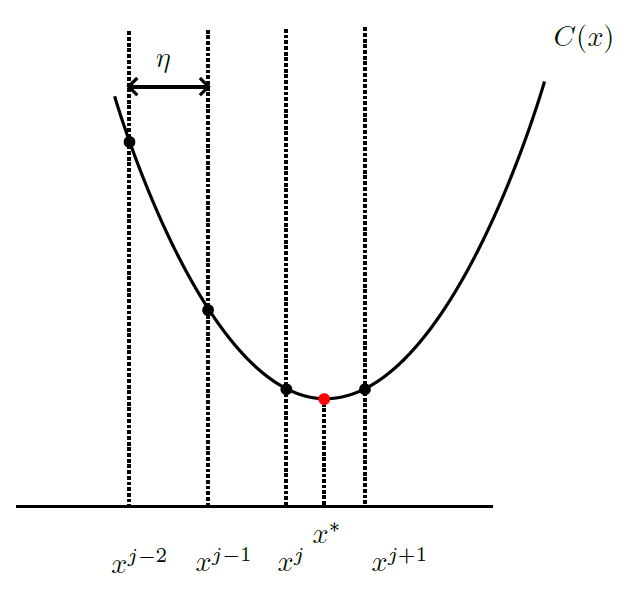
\includegraphics[scale=0.4]{../../Figures/fig_const_learning.png}
	\end{subfigure}
	\begin{subfigure}{0.4\textwidth}
		\centering
		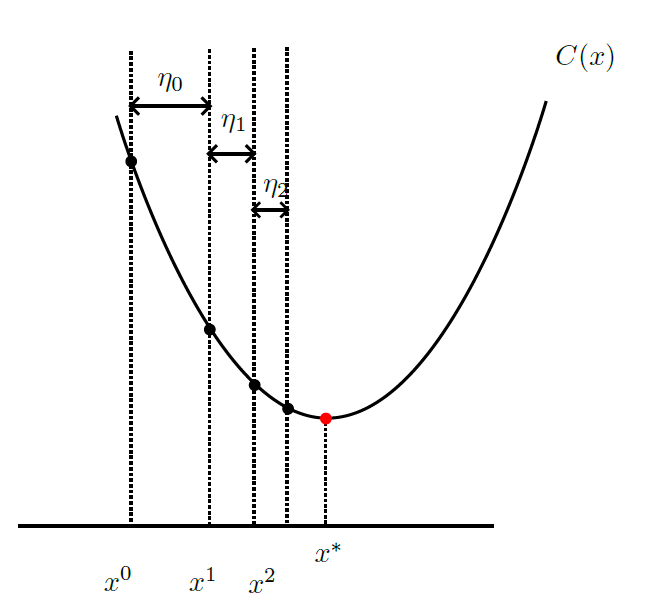
\includegraphics[scale=0.4]{../../Figures/fig_variable_learning.png}
	\end{subfigure}
\end{figure}

\end{frame}

\begin{frame}{AdaGrad}
	In 2011, Duchi et al. described a modified version of the gradient descent called \textbf{Adaptive Gradient}. 
	
	If $C(x)$ denotes the cost function ($x\in \mathbb{R}^N$), then the gradient vector $g_t= \nabla C(x(t))$.  Let $G_t$ denote the $N \times N$ matrix
	\begin{equation*}
		G_t = \sum_{j=1}^{t} g_i g_i^T
	\end{equation*}
	and consider the update
	\begin{equation*}
		x(t+1)=x(t)- \eta G_t^{-1/2} g_t
	\end{equation*}
Since $G_t^{-1/2}$ is computationally impractical in high dimension, the update can be done using only the diagonal elements of the matrix
	\begin{equation*}
	x(t+1)=x(t)- \eta \text{diag}(G_t)^{-1/2} g_t
\end{equation*}


\end{frame}

\begin{frame}{AdaGrad (cont)}
	
	
	The diagonal elements of $G_t$ can be calculated by
	\begin{equation*}
		(G_t)_{jj}= \sum_{k=1}^t (g_{kj})^2
	\end{equation*}
where 
\begin{equation*}
	g_jg_j^T= \begin{pmatrix}
		g_{j1} \\
	\vdots\\
g_{jN}
\end{pmatrix}
(g_{j1},\ldots, g_{jN}) =
\begin{pmatrix}
	(g_{j1})^2 & \cdots & \cdots \\
	\vdots & \ddots & \vdots \\
	\cdots & \cdots & (g_{jN}+)^2
\end{pmatrix}
\end{equation*}
\end{frame}

\begin{frame}{RMSProp}
	 The \textbf{Root Mean Square Propagation} or RMSProp is a variant of the gradient descent method with adaptive learning rate, which is obtained when the gradient is divided by a running average of its magnitude.
	 
	 Let $C(x)$ denote the cost function, and $g_t \nabla C(x(t))$ is the gradient evaluated at time step $t$. Then, the running average is defined recursively by
	 \begin{equation*}
	 	v(t)=\gamma v(t-1)+(1-\gamma)g_{t-1}^2,
	 \end{equation*}
	 where $\gamma\in (0,1)$ is called the \textbf{forgetting factor}, and the vector $g_{t-1}^2$ denotes the element-wise square of the gradient $g_{t-1}$. 
	 
	 It can be shown that  $v(t)$ can be expressed as
	 \begin{equation*}
	 	v(t)= \gamma^t v(0)+ (1-\gamma) \sum_{j=1}^t \gamma^{t-j}g_j^2
	 \end{equation*}
	 
\end{frame}
\begin{frame}{RMSProp}
	The minimum of the cost function $x^* = \text{arg min}_x C(x)$ is obtained by the approximation sequence $(x(t))_{t\ge 1}$ defined as
	\begin{equation*}
		x(t+1)= x(t)- \eta \frac{g_t}{\sqrt{|v(t)|}}
	\end{equation*}
where $\eta$ is the learning rate. 

One interpretation of $v$ is that it represents an estimation of the (uncentered) variance of the gradient. 
\end{frame}

\begin{frame}{Adam}
	The \textbf{Adaptive Moment Estimation} or Adam is another adaptive learning method. 
	
	\begin{fact}
		Recall that for a random variable $X$ the first and second moments are defined as $\mathbb{E}(X)$ and $\mathbb{E}(X^2)$ respectively.
	\end{fact}
	
	
	The objective is to minimize the expectation of the cost function. Namely, we look for the minimum value $x^*$ that satisfies 
	\begin{equation*}
		x^*= \text{arg min}_x \mathbb{E}(C(x))
	\end{equation*}
	In this case, we consider two exponential decay rates for the moment estimates $\beta_1,\beta_2 \in [0,1)$, and the moments updates
	
	\begin{equation*}
		\begin{split}
			m(t)&= \beta_1 m(t-1) + (1-\beta_1)g_t \\
			v(t)&=\beta_2 v(t-1)+ (1-\beta_2)(g_t)^2
		\end{split}
	\end{equation*} 	
where $m(0)=v(0)=0$.  
\end{frame}

\begin{frame}{Adam (cont)}
	We can write
	\begin{equation*}
	\begin{split}
		m(t)&= (1-\beta_1) \sum_{j=1}^t \beta_1^{t-j} g_j \\
		v(t)&=(1-\beta_2) \sum_{j=1}^t \beta_2^{t-j} (g_j)^2 
	\end{split}
\end{equation*} 		
Then, if we assume that the first and second moments are stationary  we get 
\begin{equation*}
	\begin{split}
	\mathbb{E}(m(t))=(1-\beta_1^t) \mathbb{E}(g_t) \\
		\mathbb{E}(v(t))=(1-\beta_2^t) \mathbb{E}(g_t)^2 \\
	\end{split}
\end{equation*}
Therefore, the bias-corrected moments are
\begin{equation*}
	\begin{split}
			\widehat{m}(t)&= \frac{m(t)}{1-\beta_1^t} \\
			\widehat{v}(t)&=\frac{v(t)}{1-\beta_2^t} \\
	\end{split}
\end{equation*}

\end{frame}
\begin{frame}{Adam (cont)}
	Finally, the recursive formula becomes
	\begin{equation*}
		x(t+1)= x(t)- \eta \frac{\widehat{m}(t)}{\sqrt{|\widehat{v}(t)|}+\varepsilon}
	\end{equation*}
	the $\varepsilon>0$ is a small scalar used to prevent division by zero. 
\end{frame}


\begin{frame}{References}
	Materials and some of the pictures are from \citep{calin}.
	\printbibliography 	
	
	I have used some of the graphs by hacking TiKz code from StakExchange, Inkscape for more aesthetic plots and other old tricks of \TeX
	
\end{frame}


\end{document}
